\begin{problem}{\kcpcpprobtriangle\ (\kcpcpprobtriangleshort)}
    {표준 입력}{표준 출력}
    {\kcpcpprobtriangletime\,초}{\kcpcpprobtrianglememory\,MB}{}
    
    수빈이는 원을 좋아한다. 그러나 원과 관련된 문제들이 야기하는 예외 처리 때문에 수빈이는 원에 싫증이 났고, 그 관심을 삼각형으로 옮겼다.
    
    삼각격자(triangular grid, isometric grid)에 대한 설명을 하고 넘어가자. 일반적인 $ y $축이 $ x $축과 직각을 이루는 직각좌표계와는 달리, 삼각격자는 다음 그림과 같이 $ x $축과 $ y $축이 이루는 각도가 60도이다.
    
    \begin{figure}[h]
        \centering
        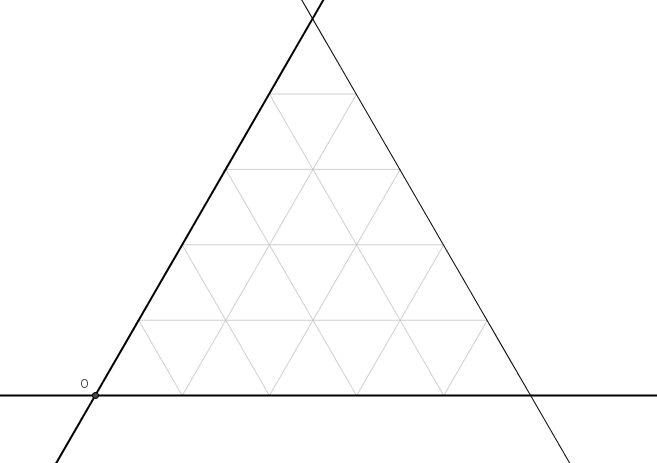
\includegraphics[height=0.25\textheight]{./problems/triangle-pic1.png}
    \end{figure}

    보이다시피, 60도라는 특성상 정삼각형이 많이 그려지는데, 이는 3개의 간단한 직선만으로 만들 수 있다. $ (0,0) $, $ (m,0) $, $ (0,m) $의 정삼각형을 만드려면 $ x=0 $, $ y=0 $, $ x+y=m $ 이 세 직선만 있으면 되기 때문이다.
    
    수학적인 호기심이 뛰어난 수빈이는 이 상태에서 세 변 중 하나에 평행하면서 이 삼각형의 내부를 지나가는 직선들을 많이 그렸다. 이를 다 그리고 나서 수빈이는 삼각격자 안에 수많은 정삼각형들이 나타난다는 것을 알아냈고, 여러분을 골탕 먹이려고 정삼각형이 몇 개가 있는지 질문을 하려고 한다.
    
    주어진 정삼각형 안에 완전히 포함되는 정삼각형이 몇 개가 만들어지는지 구하는 프로그램을 짜서 이 위기를 모면하자!
    
    \InputFile
    
    첫 번째 줄에는 정삼각형의 크기인 정수 $ m $과 수빈이가 새로 그은 직선의 개수 $ q $가 공백으로 구분되어 주어진다. ($ 1 \leq m \leq 10^9 $, $ 0 \leq q \leq min(500, 3m-3)$)
    
    정삼각형의 꼭짓점은 삼각격자에서 $ (0,0) $, $ (m,0) $, $ (0,m) $이다.
    
    그 다음 $ q $개의 줄에는 각각 두 개의 정수 $ d $와 $ l $이 공백으로 구분되어 주어진다. ($ 0 < l < m $) $ d $는 $ x $축과 이루는 각도를 의미하며, 이는 0, 60, 120 중 하나이다.
    
    \begin{itemize}
        \item $ d $가 0일 경우, 직선 $ y=l $이 추가된다.
        \item $ d $가 60일 경우, 직선 $ x=l $이 추가된다.
        \item $ d $가 120일 경우, 직선 $ x+y=l $이 추가된다. 
    \end{itemize}
    
    한 직선이 2번 이상 입력되는 경우는 없다.
    
    \OutputFile
    
    첫 번째 줄에 정삼각형들의 총 개수를 나타내는 자연수를 출력한다.
    
    \Examples
    \begin{example}
        \exmp{
            2 3
            0 1
            60 1
            120 1
        }{%
            5
        }%
         \exmp{
            10 3
            120 2
            0 1
            60 8
        }{%
            6
        }%
    \end{example}

    \Explanation
    첫 번째 예제에 대한 설명은 다음 그림에 나와 있다.
    \begin{figure}[h]
        \centering
        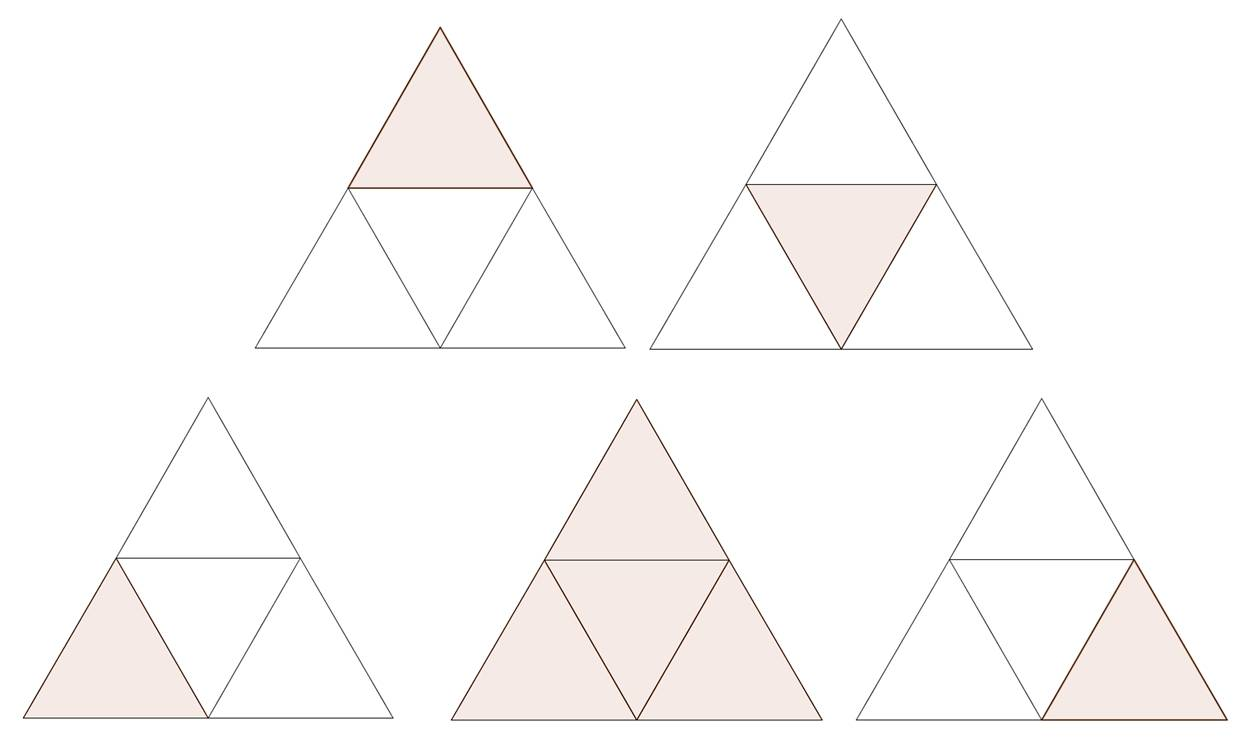
\includegraphics[height=0.25\textheight]{./problems/triangle-pic2.jpg}
    \end{figure}
    
\end{problem}

